\section{GraviDy}

\begin{frame}
    \begin{center}
        {\Huge GraviDy}
    \end{center}
\end{frame}

\begin{frame}
    \frametitle{GraviDy}
    \framesubtitle{Introduction}
    \begin{itemize}
        \item The GPU computing has been used
            in a lot of new publications related to develop N-body integrators (2012).
        \begin{itemize}
            \item Improving NBODY6 (\blue{Nitadori and Aarseth}~\cite{2012MNRAS.424..545N})
            \item New N-body codes on hybrid computing (\blue{Capuzzo-Dolcetta et al.}~\cite{2012arXiv1207.2367C})
            \item Cosmological simulations (\blue{Bard et al}~\cite{2012arXiv1208.3658B}, \blue{Bédorf et al.}~\cite{2012ASPC..453..325B})
        \end{itemize}
    \end{itemize}
\end{frame}


\begin{frame}
    \frametitle{GraviDy}
    \framesubtitle{Introduction}
    \begin{center}
        \blue{GraviDy} is a semi-Keplerian N-body integrator which aims
        to use Heterogeneous computing.
    \end{center}
\end{frame}

\begin{frame}
    \frametitle{GraviDy}
    \framesubtitle{Features}
    \begin{itemize}
        \item Based on a 4th order Hermite integrator.
        \item Using block timesteps.
        \item Includes a special treatment to work with the massive central object (\blue{On development}).
    \end{itemize}
\end{frame}

\begin{frame}
    \frametitle{GraviDy}
    \framesubtitle{Code}
    \begin{itemize}
        \item Written in C++ and CUDA.
        \item Modular developing.
    \end{itemize}
\end{frame}

\begin{frame}
    \frametitle{GraviDy}
    \framesubtitle{Predictor-Corrector procedure (Hermite 4th order)}
    \begin{enumerate}
        \item Initial $a$ and $a^{(1)}$ calculation.
        \item Initial block timesteps calculation.
        \item Select particles to move.
        \begin{enumerate}
            \item Calculate the predicted position and velocity.
            \item Calculate the $a$, $a^{(1)}$, $a^{(2)}$ and $a^{(3)}$.
            \item Apply the correction to the position and velocity.
            \item Update timesteps.
        \end{enumerate}
    \end{enumerate}
\end{frame}

\begin{frame}[fragile]
    \frametitle{GraviDy}
    \framesubtitle{Keplerian correction}
    Based on the main idea behind the integrator developed by \blue{Loeckmann and Baumgardt}~\cite{2006IAUJD...6E..24L}.
    \begin{eqnarray}
        \boldsymbol{a}_{i} =   \underbrace{ - G m_{0}
                                          \dfrac{\boldsymbol{r}_{i}}{r_{i}^{3}}
                                          }_{unperturbed\ motion}
                             - \underbrace{ \sum\limits_{\substack{j=1\\j\neq i}}^{N-1}
                                            G m_{j} \dfrac{\boldsymbol{r}_{ij}}{r_{ij}^{3}}
                                          }_{perturbing\ force}
    \end{eqnarray}
\end{frame}

\begin{frame}
    \frametitle{GraviDy}
    \framesubtitle{Kepler's correction}
    \begin{enumerate}
        \item This is applied to the \blue{Predicted} step.
        \item The normal Hermite formula is:
        \begin{eqnarray}
            \boldsymbol{r}_{pred} =    \boldsymbol{      r}_{i}              +
                                       \boldsymbol{      v}_{i} \Delta t     +
                         \dfrac{1}{2!} \boldsymbol{      a}_{i} \Delta t^{2} +
                         \dfrac{1}{3!} \boldsymbol{\dot{a}}_{i} \Delta t^{3}
        \end{eqnarray}
        \item With Kepler's correction:
        \begin{eqnarray}
            \boldsymbol{r}_{pred} =    \blue{\boldsymbol{      r}_{k,pred}}         +
                                             \boldsymbol{      v}_{i} \Delta t     +
                         \dfrac{1}{2!}       \boldsymbol{      a}_{i} \Delta t^{2} +
                         \dfrac{1}{3!}       \boldsymbol{\dot{a}}_{i} \Delta t^{3}
        \end{eqnarray}
        \item where $\boldsymbol{r}_{k}$ and its derivatives 
            are obtained from the unperturbed motion along a Keplerian orbit,
        \begin{eqnarray}
            \blue{\boldsymbol{r}_{k,pred}} =  \boldsymbol{      r}_{k}              +
                                       \boldsymbol{      v}_{k} \Delta t     +
                         \dfrac{1}{2!} \boldsymbol{      a}_{k} \Delta t^{2} +
                         \dfrac{1}{3!} \boldsymbol{\dot{a}}_{k} \Delta t^{3}
        \end{eqnarray}

    \end{enumerate}
\end{frame}

\begin{frame}
    \frametitle{Preliminary results}
    \framesubtitle{Hardware}
    \begin{itemize}
        \item GPU: Tesla C2050 (448 cores)
        \item CPU: Intel(R) Xeon(R) CPU E5504  @ 2.00GHz (4 cores)

    \end{itemize}
\end{frame}

\begin{frame}
    \frametitle{Preliminary results}
    \begin{figure}
        \centering
        \label{fig:init-time}
        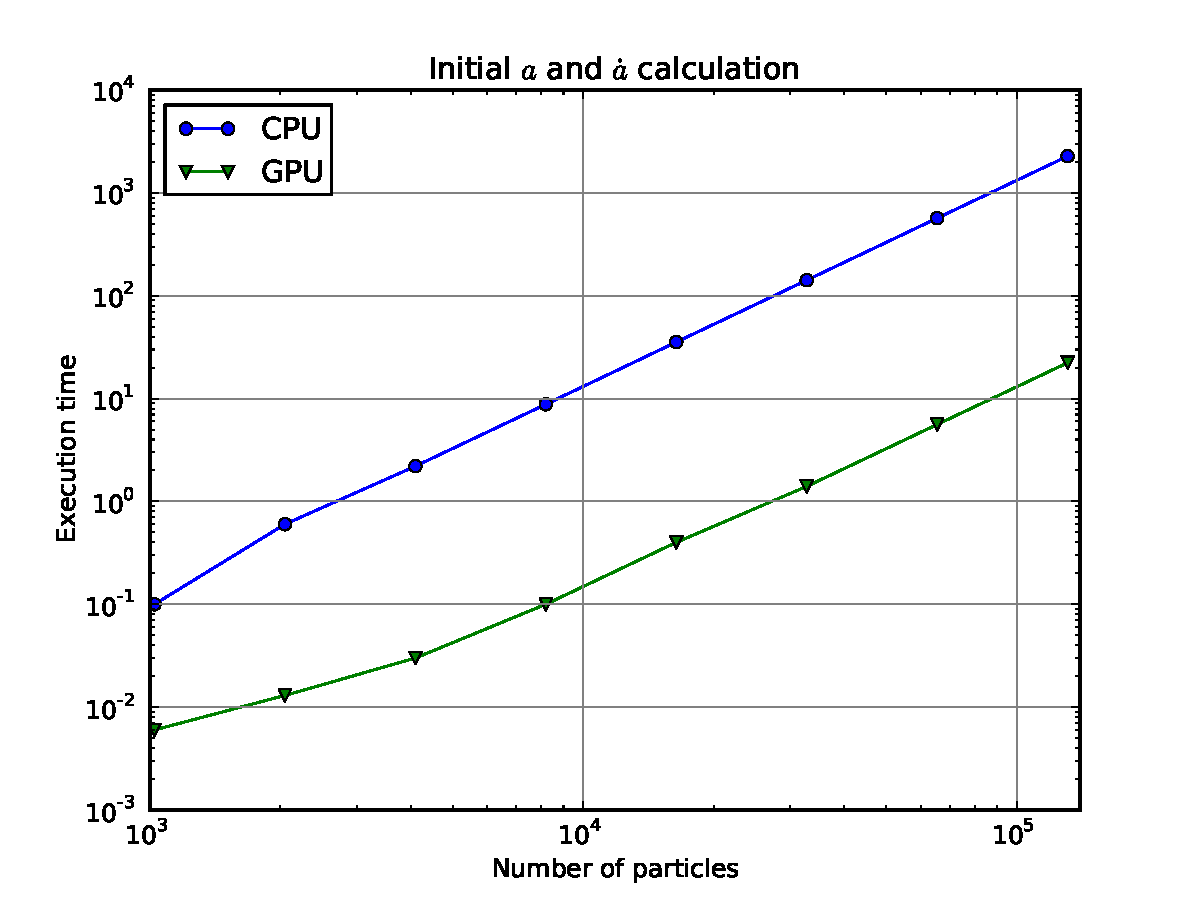
\includegraphics[width=0.7\textwidth]{img/plot-init}
        \caption{Initial $a$ and $\dot{a}$ calculation}
    \end{figure}
\end{frame}

\begin{frame}
    \frametitle{Preliminary results}
    \begin{figure}
        \centering
        \label{fig:init-time}
        %\includegraphics[width=0.8\textwidth]{img/result-init_accjerk}
        \caption{Energy Conservation}
    \end{figure}
\end{frame}

\begin{frame}
    \frametitle{Preliminary results}
    \framesubtitle{The issue related to the block timesteps scheme.}
    \begin{figure}
        \centering
        \label{fig:higpu}
        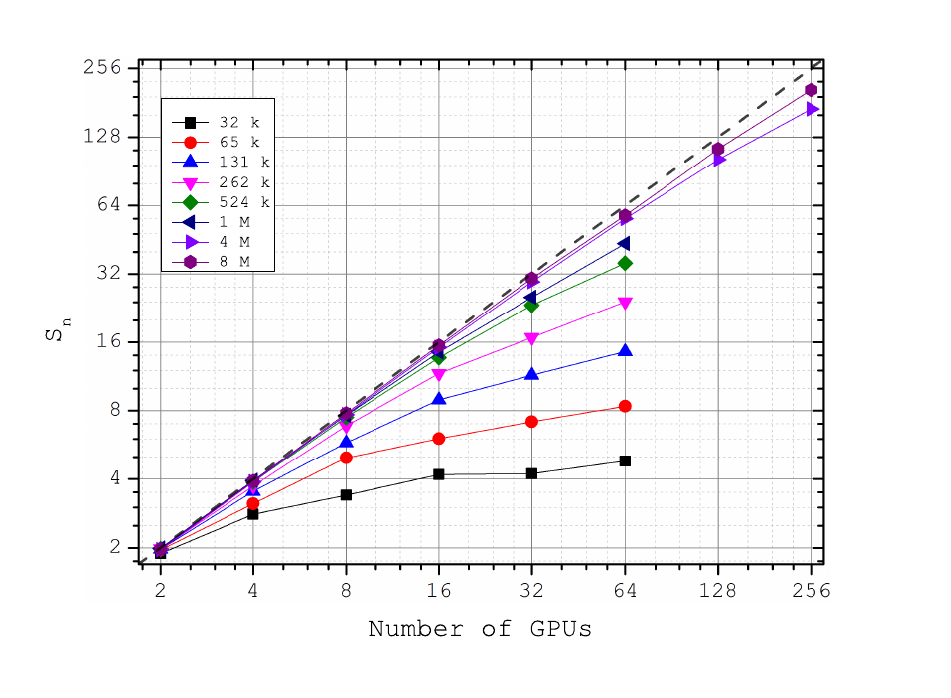
\includegraphics[width=0.6\textwidth]{img/higpu-speedup}
        \caption{Speedup as a function of the number of GPUs (\blue{Capuzzo-Dolcetta et al.} \protect \cite{2012arXiv1207.2367C})}
    \end{figure}
\end{frame}

%\begin{frame}
%    \frametitle{Preliminary results}
%    \begin{figure}
%        \centering
%        \label{fig:init-time}
%        %\includegraphics[width=0.8\textwidth]{img/result-init_accjerk}
%        \caption{Execution time}
%    \end{figure}
%\end{frame}
